\documentclass{standalone}
\usepackage{tikz}

\begin{document}
    \begin{tikzpicture}
        \draw (-1.5, 0) -- (1.5, 0);
        \draw (0, -1.5) -- (0, 1.5);
    \end{tikzpicture}

    \tikz \draw (0, 0) -- (-1, 1) -- (-1, -1) -- (1, 1);

    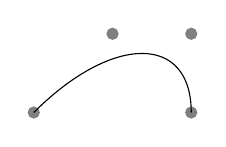
\begin{tikzpicture}
        \filldraw [gray]
        (0, 0) circle [radius=2pt]
        (1, 1) circle [radius=2pt]
        (2, 1) circle [radius=2pt]
        (2, 0) circle [radius=2pt];
        \draw (0, 0) .. controls (1, 1) and (2, 1) .. (2, 0);
    \end{tikzpicture}

    \tikz \draw (0, 0) ellipse [x radius=20pt, y radius=10pt];
    \tikz \draw [rotate=30] (0, 0) ellipse [x radius=20pt, y radius=10pt];

    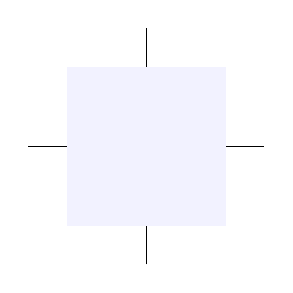
\begin{tikzpicture}
        \draw (-1.5, 0) -- (1.5, 0);
        \draw (0, -1.5) -- (0, 1.5);
        \filldraw [blue!5] (-1, -1) rectangle (1, 1);
    \end{tikzpicture}
\end{document}